You can use \texcommand{\Configure{Gin-dim}} command to change the way how image dimensions
are calculated. By default, \texfourht\ relies on information about image
dimensions provided by the Graphics package. If you use explicit dimensions
(like \texcommand{width=0.5\textwidth}), the actual dimension calculated by \TeX\ is used.

One problem is that if you set only one dimension, for example width, the other
dimension will be set to the same value. You usually don't want this, unless
your image is a square. To get the correct value for all dimensions, Graphics
uses a \verb|.xbb| file for image. It can be created using the following command:

\begin{shellcommand}
ebb -x *.jpg
\end{shellcommand}

Run analogous command for every other supported image format you use. This will
ensure that correct values are used for implicitly calculated dimensions.

\subsection{Use relative size for images}

The following configuration file example can be used to get image dimensions
relative to the original page width. Thanks to the \LaTeX\ 3 project, we can 
use the \package{l3fp} package to calculate the image dimensions in percents. 

\begin{texsource}
\Preamble{xhtml}
\makeatletter
\ExplSyntaxOn
\Configure{Gin-dim}
{style="width:\fp_eval:n{round(\Gin@req@width/\textwidth*100,2)}\char_generate:nn { `\% } { 12 }"}
\ExplSyntaxOff
\makeatother
\begin{document}
\EndPreamble
\end{texsource}

In this configuration, we divide the image width passed to
\texcommand{\includegraphics} by the document text width. 
This portion is then multiplied and rounded to get the correct percent value.
The calculated value is used in the \verb|style| attribute of the generated \verb|<img>| element.
The \package{l3fp} command \texcommand{\fp_eval:n} is used for the calculation. 
\LaTeX\ 3 is part of \LaTeX\ kernel, so we don't need to require packages that it provides.

Instead of a configuration, you can require this method using the \option{Gin-percent} option.

The following example code:

\begin{texsource}
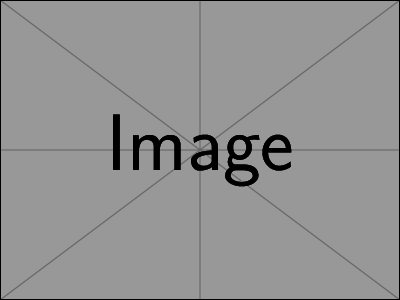
\includegraphics[width=0.5\textwidth]{example-image.png}
\end{texsource}

produces following HTML code:

\begin{htmlsource}
<img style='width:50%' alt='PIC' src='example-image.png' />
\end{htmlsource}

You can also require the above method using the \option{Gin-percent}
option.

To disable setting of the image dimensions in HTML code completely
use the following configuration:

\begin{texsource}
\Preamble{xhtml}
\Configure{Gin-dim}{}
\Css{img {
    max-width: 100\%;
    height: auto;
}}
\begin{document}
\EndPreamble
\end{texsource}

This configuration uses CSS to set the maximum image dimension. This ensures that
the image is donwsized on devices smaller than is the actual image size.


\subsection{Change image's alternative text}

The \package{Graphicx} package recently added alternative text support,
which can be used to describe the image. This is necessary
for the accessibility purposes.

If you use an older system, without support for this attribute, 
you can use the following example to define it yourself, and use it 
with the \texcommand{\includegraphics} command. The attribute is named 
\texttt{alt}. Here is a sample file that shows how to do that:

\texinput{examples/imagealt/sample.tex}

The \texcommand{\define@key{Gin}{alt}{}} command defines a dummy command that
is used by regular \LaTeX. We need to redefine this key for \texfourht, so it uses the
configuration that can specify the image alternative text, \configuration{GraphicsAlt}.

\texinput{examples/imagealt/mycfg.cfg} 

The resulting HTML file now contains image with the \texttt{alt} attribute:

\htmlinput{examples/imagealt/sample-body.html}
